% Options for packages loaded elsewhere
\PassOptionsToPackage{unicode}{hyperref}
\PassOptionsToPackage{hyphens}{url}
%
\documentclass[
]{book}
\usepackage{amsmath,amssymb}
\usepackage{lmodern}
\usepackage{ifxetex,ifluatex}
\ifnum 0\ifxetex 1\fi\ifluatex 1\fi=0 % if pdftex
  \usepackage[T1]{fontenc}
  \usepackage[utf8]{inputenc}
  \usepackage{textcomp} % provide euro and other symbols
\else % if luatex or xetex
  \usepackage{unicode-math}
  \defaultfontfeatures{Scale=MatchLowercase}
  \defaultfontfeatures[\rmfamily]{Ligatures=TeX,Scale=1}
\fi
% Use upquote if available, for straight quotes in verbatim environments
\IfFileExists{upquote.sty}{\usepackage{upquote}}{}
\IfFileExists{microtype.sty}{% use microtype if available
  \usepackage[]{microtype}
  \UseMicrotypeSet[protrusion]{basicmath} % disable protrusion for tt fonts
}{}
\makeatletter
\@ifundefined{KOMAClassName}{% if non-KOMA class
  \IfFileExists{parskip.sty}{%
    \usepackage{parskip}
  }{% else
    \setlength{\parindent}{0pt}
    \setlength{\parskip}{6pt plus 2pt minus 1pt}}
}{% if KOMA class
  \KOMAoptions{parskip=half}}
\makeatother
\usepackage{xcolor}
\IfFileExists{xurl.sty}{\usepackage{xurl}}{} % add URL line breaks if available
\IfFileExists{bookmark.sty}{\usepackage{bookmark}}{\usepackage{hyperref}}
\hypersetup{
  pdftitle={Varia},
  pdfauthor={Dyrehaugen Web Notebook},
  hidelinks,
  pdfcreator={LaTeX via pandoc}}
\urlstyle{same} % disable monospaced font for URLs
\usepackage{longtable,booktabs,array}
\usepackage{calc} % for calculating minipage widths
% Correct order of tables after \paragraph or \subparagraph
\usepackage{etoolbox}
\makeatletter
\patchcmd\longtable{\par}{\if@noskipsec\mbox{}\fi\par}{}{}
\makeatother
% Allow footnotes in longtable head/foot
\IfFileExists{footnotehyper.sty}{\usepackage{footnotehyper}}{\usepackage{footnote}}
\makesavenoteenv{longtable}
\usepackage{graphicx}
\makeatletter
\def\maxwidth{\ifdim\Gin@nat@width>\linewidth\linewidth\else\Gin@nat@width\fi}
\def\maxheight{\ifdim\Gin@nat@height>\textheight\textheight\else\Gin@nat@height\fi}
\makeatother
% Scale images if necessary, so that they will not overflow the page
% margins by default, and it is still possible to overwrite the defaults
% using explicit options in \includegraphics[width, height, ...]{}
\setkeys{Gin}{width=\maxwidth,height=\maxheight,keepaspectratio}
% Set default figure placement to htbp
\makeatletter
\def\fps@figure{htbp}
\makeatother
\setlength{\emergencystretch}{3em} % prevent overfull lines
\providecommand{\tightlist}{%
  \setlength{\itemsep}{0pt}\setlength{\parskip}{0pt}}
\setcounter{secnumdepth}{5}
\usepackage{booktabs}
\usepackage{amsthm}
\makeatletter
\def\thm@space@setup{%
  \thm@preskip=8pt plus 2pt minus 4pt
  \thm@postskip=\thm@preskip
}
\makeatother

\renewcommand\chaptername{}
\ifluatex
  \usepackage{selnolig}  % disable illegal ligatures
\fi
\usepackage[]{natbib}
\bibliographystyle{apalike}

\title{Varia}
\author{Dyrehaugen Web Notebook}
\date{2021-02-03}

\begin{document}
\maketitle

{
\setcounter{tocdepth}{1}
\tableofcontents
}
\hypertarget{varia}{%
\chapter{Varia}\label{varia}}

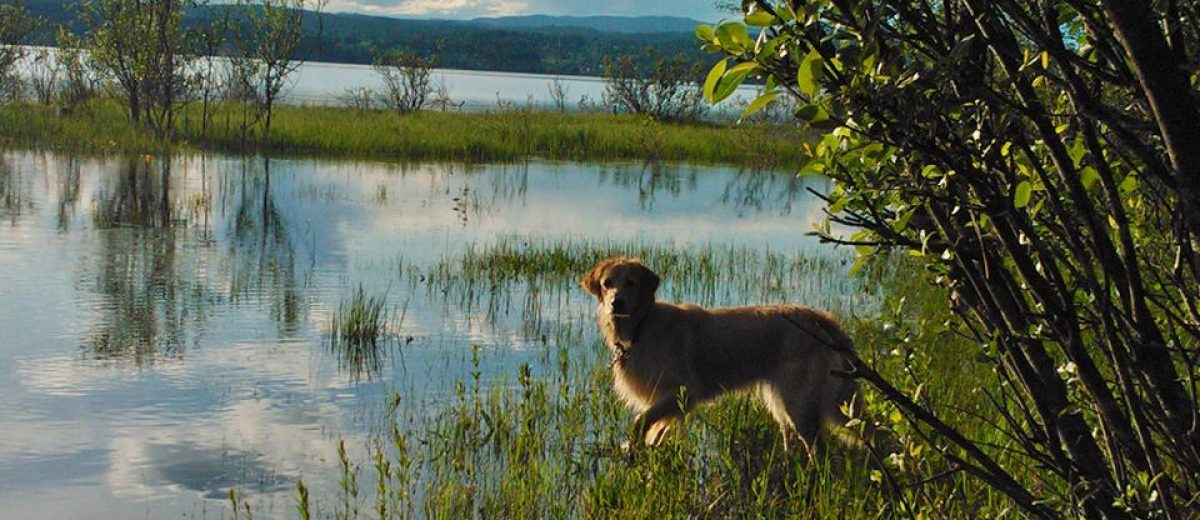
\includegraphics{fig/zelda.jpg}

\hypertarget{statistics}{%
\chapter{Statistics}\label{statistics}}

\href{/pdf/statistics.pdf}{(pdf)}

\begin{verbatim}
Statistics
Fat Tails
    Extremes      
        Catastrophe Principle  
    Statistical Consequences of Fat Tails  
    Power Law Distributions  
        Pareto Distribution  
    Pandemic Risk Management
\end{verbatim}

Science uses statistics \&, as per Popper, doesn't really ``accept'',
just fails to reject at some significance.
It's fundamentally disconfirmatory.
Stat. ``evidence'' is inherently probabilistic and
cannot be ``degenerate'' (i.e.~provide certainties).
(Taleb)

\hypertarget{fat-tails}{%
\section{Fat Tails}\label{fat-tails}}

\hypertarget{extremes}{%
\subsection{Extremes}\label{extremes}}

The field of Extreme Value Theory focuses on tail properties,
not the mean or statistical inference.

It is vastly more effective
to focus on being insulated from the harm of random events
than try to figure them out in the required details
(the inferential errors under fat tails are huge).
So it is more solid, much wiser, more ethical, and more effective to focus on
detection heuristics and policies rather than fabricate statistical properties.

\hypertarget{catastrophe-principle}{%
\subsubsection{Catastrophe Principle}\label{catastrophe-principle}}

\emph{Memo Taleb (DarwinCollege):}

Where a Pareto distribution
prevails (among many), and randomly select two people with
combined wealth of £36 million. The most likely combination
is not £18 million and £18 million. It is approximately
£35,999,000 and £1,000. This highlights the crisp distinction
between the two domains; for the class of subexponential
distributions, \emph{ruin is more likely to come from a single extreme
event than from a series of bad episodes}. This logic underpins
classical risk theory as outlined by Lundberg early in the 20 th
Century and formalized by Cramer, but forgotten by
economists in recent times. This indicates that insurance can
only work in Medocristan; you should never write an uncapped
insurance contract if there is a risk of catastrophe. The point
is called the catastrophe principle.

Cramer showed insurance could not work outside
what he called the Cramer condition, which excludes possible
ruin from single shocks.

With fat tail distributions, extreme events
away from the centre of the distribution play a very large
role. Black swans are not more frequent, they are more
consequential. The fattest tail distribution has just one very
large extreme deviation, rather than many departures form the
norm.

There are three types of fat tails based on mathematical properties.

First there are entry level fat tails.
This is any distribution with fatter tails than the Gaussian
i.e.~with more observations within one sigma and with
kurtosis (a function of the fourth central moment) higher than three.

Second, there are subexponential distributions.

\emph{LogNormal:}

The subexponential class includes the lognormal, which is one
of the strangest things on earth because sometimes it cheats
and moves up to the top of the diagram. At low variance, it is
thin-tailed, at high variance, it behaves like the very fat tailed.
in-tailed, at high variance, it behaves like the very fat tailed.

Membership in the subexponential class satisfies the Cramer
condition of possibility of insurance (losses are more likely to
come from many events than a single one)
Technically it means that the expectation of
the exponential of the random variable exists.

Third, what is called by a variety of names, the power law, or slowly
varying class, or ``Pareto tails'' class correspond to real fat tails.

The traditional statisticians approach to fat tails has been
to assume a different distribution but keep doing business as
usual, using same metrics, tests, and statements of significance.
But this is not how it really works and they fall into logical
inconsistencies.

Once we are outsaide the zone for which statistical techniques were designed,
things no longer work as planned.
Here are some consequences

\begin{enumerate}
\def\labelenumi{\arabic{enumi})}
\item
  The law of large numbers, when it works, works too slowly in the real
  world (this is more shocking than you think as it cancels most statistical estimators)
\item
  The mean of the distribution will not correspond to the sample mean.\\
  In fact, there is no fat tailed distribution in which the mean can be properly
  estimated directly from the sample mean,
  unless we have orders of magnitude more data than we do
\item
  Standard deviations and variance are not useable. They fail out of sample.
\item
  Beta, Sharpe Ratio and other common financial metrics
  are uninformative.
\item
  Robust statistics is not robust at all.
\item
  The so-called ``empirical distribution'' is not empirical
  (as it misrepresents the expected payoffs in the tails).
\item
  Linear regression doesn't work.
\item
  Maximum likelihood methods work for parameters
  (good news). We can have plug in estimators in some
  situations.
\item
  The gap between dis-confirmatory and confirmatory
  empiricism is wider than in situations covered by common
  statistics i.e.~difference between absence of evidence and
  evidence of absence becomes larger.
\item
  Principal component analysis is likely to produce false
  factors.
\item
  Methods of moments fail to work. Higher moments are
  uninformative or do not exist.
\item
  There is no such thing as a typical large deviation:
  conditional on having a large move, such move is not
  defined.
\item
  The Gini coefficient ceases to be additive. It becomes
  super-additive. The Gini gives an illusion of large con-
  centrations of wealth. (In other words, inequality in a
  continent, say Europe, can be higher than the average
  inequality of its members).
\end{enumerate}

While it takes 30 observations in the Gaussian to stabilize
the mean up to a given level,
it takes \(10^{11}\) observations in the Pareto to bring the sample error down
by the same amount (assuming the mean exists).
You cannot make claims about the stability of the sample
mean with a fat tailed distribution. There are other ways to do
this, but not from observations on the sample mean.

We have known at least since Sextus Empiricus that we
cannot rule out degeneracy but there are situations in which
we can rule out non-degeneracy. If I see a distribution that
has no randomness, I cannot say it is not random. That is,
we cannot say there are no black swans. Let us now add
one observation. I can now see it is random, and I can
rule out degeneracy. I can say it is not not random. On the
right hand side we have seen a black swan, therefore the
statement that there are no black swans is wrong. This is the
negative empiricism that underpins Western science. As we
gather information, we can rule things out.
If we see a 20 sigma event, we can rule out that the
distribution is thin-tailed.

\emph{Pareto - Scalability}

The intuition behind the Pareto Law. It is simply defined as:
say X is a random variable.
For x sufficently large, the probability of exceeding 2x divided by the
probability of exceeding x is no different from the probability
of exceeding 4x divided by the probability of exceeding 2x,
and so forth.

So if we have a Pareto (or Pareto-style) distribution, the ratio
of people with £16 million compared to £8 million is the same
as the ratio of people with £2 million and £1 million. There
is a constant inequality.

This distribution has no characteristic
scale which makes it very easy to understand. Although this
distribution often has no mean and no standard deviation we
still understand it. But because it has no mean we have to
ditch the statistical textbooks and do something more solid,
more rigorous.

A Pareto distribution has no higher moments: moments
either do not exist or become statistically more and more
unstable.

In 2009 I took 55 years of data and
looked at how much of the kurtosis (a function of the fourth
moment) came from the largest observation. For
a Gaussian the maximum contribution over the same time span
should be around .008 ± .0028. For the S\&P 500 it was about
80 per cent. This tells us that we dont know anything about
kurtosis. Its sample error is huge; or it may not exist so the
measurement is heavily sample dependent. If we dont know
anything about the fourth moment, we know nothing about the
stability of the second moment. It means we are not in a class
of distribution that allows us to work with the variance, even
if it exists. This is finance.

We cannot use standard statistical methods with financial data.

Financial data, debunks all the college textbooks we are currently using
Econometrics that deals with squares goes out of the window.
The variance of the squares is analogous to the fourth moment.
The variance of the squares is analogous to the fourth moment.
We do not know the variance. But we can work very easily
with Pareto distributions. They give us less information, but
nevertheless, it is more rigorous if the data are uncapped or if
there are any open variables.

Principal component analysis is a dimension
reduction method for big data and it works beautifully with
thin tails. But if there is not enough data there is an illusion
of a structure. As we increase the data (the n variables),
the structure becomes flat.

\emph{Lessons:}

Once we know something is fat-tailed, we can use heuristics to see
how an exposure there reacts to random events: how much
is a given unit harmed by them. It is vastly more effective
to focus on being insulated from the harm of random events
than try to figure them out in the required details (as we saw
the inferential errors under fat tails are huge). So it is more
solid, much wiser, more ethical, and more effective to focus on
detection heuristics and policies rather than fabricate statistical
properties.

The beautiful thing we discovered is that everything that is
fragile has to present a concave exposure similar --if not
identical --to the payoff of a short option, that is, a negative
exposure to volatility. It is nonlinear, necessarily. It has to
have harm that accelerates with intensity, up to the point of
breaking. If I jump 10m I am harmed more than 10 times than
if I jump one metre. That is a necessary property of fragility.

We just need to look at acceleration in the tails. We have built
effective stress testing heuristics based on such an option-like
property.

In the real world we want simple things that work;
we want to impress our accountant and not our peers. (My
argument in the latest instalment of the Incerto, Skin in the
Game is that systems judged by peers and not evolution rot
from overcomplication). To survive we need to have clear
techniques that map to our procedural intuitions.

The new focus is on how to detect and measure convexity and concavity.
This is much, much simpler than probability.

\href{/pdf/Taleb_2017_Extremes_DarwinCollege.pdf}{Taleb (2017) Darwin Colleges(pdf)}

\hypertarget{statistical-consequences-of-fat-tails}{%
\subsubsection{Statistical Consequences of Fat Tails}\label{statistical-consequences-of-fat-tails}}

\begin{quote}
Conventional statistics fail to cover fat tails;
physicists who use power laws do not usually produce statistical estimators.
\end{quote}

\href{https://www.fooledbyrandomness.com/FatTails.html}{Taleb's Research Site}

\begin{quote}
Take nothing for granted - \emph{It is what it is.}
Another 300 years of data is required to test a statistical hypothesis.
A dataset has no variance.
A distribution's standard deviation will not converge in a lifetime's worth of data.
\end{quote}

Fat tailed random variables challenge our conceptions of mean and standard deviation.
Linear regression also breaks under fat tails.
The convincing case is made that power law distributions should be the default
for modeling data rather than the thin-tailed Normal distribution.

Any distribution with more density in the tails than the Normal distribution
is said to have thick tails.
This corresponds to raw kurtosis \textgreater{} 3.
The tail density needs to decay slower than Normal, \(\frac{-x^2}{e^{2\sigma^2}}\).

Fat tailed distributions are the thickest tailed distributions.
The power law is an example of this -
they're the distributions with so much additional density in their tails
that moments \(E[X^p]\) are no longer finite.

\hypertarget{power-law-distributions}{%
\subsubsection{Power Law Distributions}\label{power-law-distributions}}

\hypertarget{pareto-distribution}{%
\paragraph{Pareto Distribution}\label{pareto-distribution}}

Pareto discovered that 20\% percent of taxpayers had 80\% of the income across countries in Europe.
One parameter of the Pareto power law distribution is α, which is known as the \emph{tail index}.
Pareto's 80-20 example corresponds to α = 1.16.
The tail index describes the behavior of density decay in the tail, as its name implies.

The strange thing about power law distributions is that, depending on the tail index α,
some of its moments may not exist or be infinite.
There is no finite mean if α \textless{} 1,
and there is no finite variance if α \textless{} 2.
The same applies for skewness at α \textless{} 3 and kurtosis when α \textless{} 4, and so on.
The tails get thicker as α gets smaller.

Pseudo-convergence: A tail index less than 2 doesn't mean that we can't compute the sample variance of dataset. Rather, betting on the stability of the variance is unwise because this sample variance will never converge, and can in fact ``spike'' at any time. Furthermore, if the 4th moment (kurtosis) doesn't exist, this may imply unbearably slow convergence of the 2nd moment (variance).

The Central Limit Theorem, which is typically very useful for sums and averages, requires a finite variance, so tail indices α \textless{} 2 do not obey. The assumption for the analytic Black-Scholes-Merton price for a financial option - that the random walk sum of movements converges to the Normal distribution - is also violated, so that breaks too. If the tail index is slightly over 2, it will converge to the Normal in the limit, but very slowly.

\emph{Tail events} - the unlikely events of the atypically large magnitude - are the most indicative of the tail behavior. But these tail events are rare. Without a deep understanding of the underlying process which has generated these samples, it can be tough to rule out that the data was generated by a power law. In this sense, we might consider that ``most'' processes are fat tailed by default - or, we should at least assume they are until we have enough quantitative or qualitative data to prove otherwise.

\href{https://gelman.me/scoft.html}{Review of Taleb (Gelman)}

\hypertarget{pandemic-risk-management}{%
\subsection{Pandemic Risk Management}\label{pandemic-risk-management}}

\emph{Non-Ergodic}

\emph{Paranoia or Nothing}

Taleb and collegues have som very interesting methodological
remarks in the early stages of the COVID-19 outbreak:

\begin{quote}
Clearly, we are dealing with an extreme fat-tailed process
owing to an increased connectivity, which increases the
spreading in a nonlinear way. Fat tailed processes
have special attributes, making conventional risk-management
approaches inadequate
\end{quote}

\begin{quote}
The general (non-naive) precautionary principle delin-
eates conditions where actions must be taken to reduce risk
of ruin, and traditional cost-benefit analyses must not be used.
These are ruin problems where, over time, exposure to tail
events leads to a certain eventual extinction. While there
is a very high probability for humanity surviving a single
such event, over time, there is eventually zero probability of
surviving repeated exposures to such events. While repeated
risks can be taken by individuals with a limited life expectancy,
ruin exposures must never be taken at the systemic and
collective level. In technical terms, the precautionary principle
applies when traditional statistical averages are invalid because
risks are not ergodic.
\end{quote}

\begin{quote}
Historically based estimates of spreading
rates for pandemics in general, and for the current one in
particular, underestimate the rate of spread because of the
rapid increases in transportation connectivity over recent years.
This means that expectations of the extent of harm are under-
estimates both because events are inherently fat tailed, and
because the tail is becoming fatter as connectivity increases
\end{quote}

\begin{quote}
Estimates of the virus's reproductive
ratio \(R\_{0}\) ---the number of cases one case generates on average
over the course of its infectious period in an otherwise
uninfected population---are biased downwards. This property
comes from fat-tailedness due to individual `superspreader'
events. Simply,\(R\_{0}\) is estimated from an average which takes
longer to converge as it is itself a fat-tailed variable.
\end{quote}

\href{https://necsi.edu/systemic-risk-of-pandemic-via-novel-pathogens-coronavirus-\%20a-note}{Norman/Bar-Yam/Taleb Note}
\href{/pdf/Joseph_Norman_2020_Systemic_Risk_of_Pandemic_via_Novel_Pathogenes.pdf}{(pdf)}

\hypertarget{entropy}{%
\chapter{Entropy}\label{entropy}}

\hypertarget{information-entropy---shannon}{%
\section{Information Entropy - Shannon}\label{information-entropy---shannon}}

In a single groundbreaking paper, he laid the foundation for the entire communication infrastructure underlying the modern information age.

The heart of his theory is a simple but very general model of communication: A transmitter encodes information into a signal, which is corrupted by noise and then decoded by the receiver. Despite its simplicity, Shannon's model incorporates two key insights: isolating the information and noise sources from the communication system to be designed, and modeling both of these sources probabilistically. He imagined the information source generating one of many possible messages to communicate, each of which had a certain probability. The probabilistic noise added further randomness for the receiver to disentangle.

Before Shannon, the problem of communication was primarily viewed as a deterministic signal-reconstruction problem: how to transform a received signal, distorted by the physical medium, to reconstruct the original as accurately as possible. Shannon's genius lay in his observation that the key to communication is uncertainty.
This single observation shifted the communication problem from the physical to the abstract, allowing Shannon to model the uncertainty using probability. This came as a total shock to the communication engineers of the day.

First, Shannon came up with a formula for the minimum number of bits per second to represent the information, a number he called its entropy rate, H. This number quantifies the uncertainty involved in determining which message the source will generate. The lower the entropy rate, the less the uncertainty, and thus the easier it is to compress the message into something shorter.

For example, texting at the rate of 100 English letters per minute means sending one out of 26100 possible messages every minute, each represented by a sequence of 100 letters. One could encode all these possibilities into 470 bits, since 2470 ≈ 26100. If the sequences were equally likely, then Shannon's formula would say that the entropy rate is indeed 470 bits per minute. In reality, some sequences are much more likely than others, and the entropy rate is much lower, allowing for greater compression.

Second, he provided a formula for the maximum number of bits per second that can be reliably communicated in the face of noise, which he called the system's capacity, C. This is the maximum rate at which the receiver can resolve the message's uncertainty, effectively making it the speed limit for communication.

Finally, he showed that reliable communication of the information from the source in the face of noise is possible if and only if H \textless{} C. Thus, information is like water: If the flow rate is less than the capacity of the pipe, then the stream gets through reliably.

His theorems led to some counterintuitive conclusions. Suppose you are talking in a very noisy place. What's the best way of making sure your message gets through? Maybe repeating it many times? That's certainly anyone's first instinct in a loud restaurant, but it turns out that's not very efficient. Sure, the more times you repeat yourself, the more reliable the communication is. But you've sacrificed speed for reliability. Shannon showed us we can do far better. Repeating a message is an example of using a code to transmit a message, and by using different and more sophisticated codes, one can communicate fast --- all the way up to the speed limit, C --- while maintaining any given degree of reliability.

Another unexpected conclusion stemming from Shannon's theory is that whatever the nature of the information --- be it a Shakespeare sonnet, a recording of Beethoven's Fifth Symphony or a Kurosawa movie --- it is always most efficient to encode it into bits before transmitting it. So in a radio system, for example, even though both the initial sound and the electromagnetic signal sent over the air are analog wave forms, Shannon's theorems imply that it is optimal to first digitize the sound wave into bits, and then map those bits into the electromagnetic wave. This surprising result is a cornerstone of the modern digital information age, where the bit reigns supreme as the universal currency of information.

Shannon's general theory of communication is so natural that it's as if he discovered the universe's laws of communication, rather than inventing them. His theory is as fundamental as the physical laws of nature. In that sense, he was a scientist.

Shannon invented new mathematics to describe the laws of communication. He introduced new ideas, like the entropy rate of a probabilistic model, which have been applied in far-ranging branches of mathematics such as ergodic theory, the study of long-term behavior of dynamical systems. In that sense, Shannon was a mathematician.

Shannon's theory has now become the standard framework underlying all modern-day communication systems: optical, underwater, even interplanetary.

Shannon figured out the foundation for all this more than 70 years ago. How did he do it? By focusing relentlessly on the essential feature of a problem while ignoring all other aspects.

\href{https://www.quantamagazine.org/how-claude-shannons-information-theory-invented-the-future-20201222/}{Shannon (Quanta Magazine)}

\hypertarget{economics}{%
\chapter{Economics}\label{economics}}

\href{/docs/behavioural}{Behavioural Economics}

\hypertarget{behavioral-economics}{%
\section{Behavioral Economics}\label{behavioral-economics}}

\hypertarget{fooled-by-randomness}{%
\subsection{Fooled by randomness}\label{fooled-by-randomness}}

\emph{Memo}

There is strong evidence from the lab that people have misperceptions about what randomness looks like. When a person is asked to generate a series that approximates the flipping of a coin, they will alternate between heads and tails too often, and balance the frequencies of heads and tails over too short a sequence. When people are asked to judge which of two different sequences of coin flips are more likely, they tend to pick sequences with more alternation, despite their probability being the same.

What happens we look for a failure to perceive randomness in the outside world? Out of the lab?

When people watch basketball, they often see a hot hand. They will describe players as ``hot'' and ``in form''. Their belief is that the person who has just hit a shot or a series of shots is more likely to hit their next one.

But is this belief in the ``hot hand'' a rational belief? Or is the hot hand an illusion, whereby, just like they do with coins, they are seeing streaks in what is actually randomness?

In a famous examination of this question, Thomas Gilovich, Robert Vallone and Amos Tversky took shot data from a variety of sources, including the Philadelphia 76ers and Boston Celtics, and examined it for evidence of a hot hand.

What did they find? The hot hand was an illusion. As Daniel Kahneman wrote in Thinking, Fast and Slow when describing this research:

\begin{quote}
The hot hand is entirely in the eye of the beholders, who are consistently too quick to perceive order and causality in randomness. The hot hand is a massive and widespread cognitive illusion.
\end{quote}

Possibly even more interesting was the reaction to the findings from those in the sporting world. Despite the analysis, many sports figures denied that it could be true. Red Auerbach, who coached the Boston Celtics to nine NBA championships, said ``Who is this guy? So he makes a study. I couldn't care less.''

This provides another insight, about which Gilovich wrote:

\begin{quote}
The story of our research on the hot hand is only partly about the misperception of random events. It is also about how tenaciously people cling to their beliefs even in the face of hostile evidence.
\end{quote}

So, this isn't just about the misperception of the hot hand, but also about the failure of people to see their error when presented with evidence about it.

Let's delve into how Gilovich, Vallone and Tversky showed the absence of a hot hand.

Imagine a person who took ten shots in a basketball game. A ball is a hit, an X is a miss.

What would count as evidence of a hot hand? What we can do is look at shots following a previous hit. For instance, in this sequence of shots there are 6 occasions where we have a shot following a previous hit. Five of those shots, such as the seventh here, are followed by another hit.

We can then compare their normal shooting percentage with the proportion of shots they hit if the shot immediately before was a hit. If their hit rate after a hit is higher than their normal shot probability, then we might say they get a hot hand.

This is effectively how Gilovich, Vallone and Tversky examined the hot hand in coming to their conclusion that it doesn't exist. They also looked at whether there was a hit or miss after longer streaks of hits or misses, but this captures the basic methodology. It seems sensible.

But let me take a detour that involves flipping a coin.

Suppose you flip a coin three times. Here are the eight possible sequences of heads and tails. Each sequence has an equal probability of occurring. What if I asked you: if you were to flip a coin three times, and there is a heads followed by another flip in that sequence, what is the expected probability that another heads will follow that heads?

Here is the proportion of heads following a previous flip of heads for each sequence. In the first row of the table, the first flip is a head. That first flip is followed by another head. After the second flip, a head, we also have a head. There is no flip after the third head. 100\% of the heads in that sequence followed by another flip are followed by a head.

In the second row of the table, 50\% of the heads are followed by a head. In the last two rows, there are no heads followed by another flip.

Now, back to our question: if you were to flip a coin three times, and there is a heads followed by another flip in that sequence, what is the expected probability that another heads will follow that heads? It turns out it is 42\%, which I can get by averaging those proportions.

8 possible combinations of heads and tails across three flips

\begin{longtable}[]{@{}ll@{}}
\toprule
Flips & p(Ht+1\textbar Ht) \\ \addlinespace
\midrule
\endhead
HHH & 100\% \\ \addlinespace
HHT & 50\% \\ \addlinespace
HTH & 0\% \\ \addlinespace
HTT & 0\% \\ \addlinespace
THH & 100\% \\ \addlinespace
THT & 0\% \\ \addlinespace
TTH & -- \\ \addlinespace
TTT & -- \\ \addlinespace
Exp.val & 42\% \\ \addlinespace
\bottomrule
\end{longtable}

That doesn't seem right. If we count across all the sequences, we see that there are 8 flips of heads that are followed by another flip. Of the subsequent flips, 4 are heads and 4 are tails, spot on the 50\% you expect.

What is going on in that second column? By looking at these short sequences, we are introducing a bias. The cases of heads following heads tend to cluster together, such as in the first sequence which has two cases of a heads following a heads. Yet the sequence THT, which has only one shot occurring after a heads, is equally likely to occur. The reason a tails appears more likely to follow a heads is because of this bias whereby the streaks tend to cluster together. The expected value I get when taking a series of three flips is 42\%, when in fact the actual probability of a heads following a heads is 50\%. As the sequence of flips gets longer, the size of the bias is reduced, although it is increased if we examine longer streaks, such as the probability of a heads after three previous heads.

Why have I bothered with this counterintuitive story about coin flipping?

Because this bias is present in the methodology of the papers that purportedly demonstrated that there was no hot hand in basketball. Because of this bias, the proportion of hits following a hit or sequence of hits is biased downwards. Like our calculation using coins, the expected proportion of hits following a hit in a sequence is lower than the actual probability of hitting a shot.

Conversely the hot hand pushes the probability of hitting a shot after a previous hit up. Together, the downward bias and the hot hand roughly cancelled each other out, leading to the conclusion by researchers that each shot is independent of the last.

The result is, that when you correct for the bias, you can see that there actually is a hot hand in basketball.

When Miller and Sanjurjo crunched the numbers for one of the studies in the Gilovich and friends paper, they found that the probability of hitting a shot following a sequence of three previous hits is 13 percentage points higher than after a sequence of three misses. There truly is a hot hand. If Red Auerbach had coached as though there were no hot hand, what would his record have looked like?

I should say, this point does not debunk the earlier point about people misperceiving randomness. The lab evidence is strong. People tend to see the hot hand when people flip coins. It is possible that people overestimate the strength of the hot hand in the wild, although that is hard to show. But the hot hand exists.

Let's turn back to one of the quotes I showed earlier.

\begin{quote}
The story of our research on the hot hand is only partly about the misperception of random events. It is also about how tenaciously people cling to their beliefs even in the face of hostile evidence.
\end{quote}

The researchers expanded the original hot hand research from a story about people misperceiving randomness, to one of them continuing to do so even when presented with evidence that they were making an error.

But, as we can now see, their belief in the hot hand was not an error. The punters in the stands were right. Their accumulated experience had given them the answer. The researchers were wrong. Rather than the researchers asking whether they themselves were making an error when people refused to believe their research, they double downed and identified a second failure of human reasoning. The blunt dismissal of people's beliefs led behavioural scientists to hold an untrue belief for over thirty years

This is a persistent characteristic of much applied behavioural science. It was an error I made many times when I first came to the discipline. We spend too little time questioning our understanding of the decisions or observations other people make. If we believe they are in error, we should first question whether the error is ours.

\href{https://jasoncollins.blog/2020/06/12/arent-we-smart-fellow-behavioural-scientists/}{Jason Collins on Nudgestock 2020}

\hypertarget{climate-finance}{%
\section{Climate Finance}\label{climate-finance}}

Climate Finance assistance to developing countries is NOT on track.
\href{/docs/news/\#210102-climate-finance-shadow-report-2020}{Oxfam Report 2020 (News issue)}

\hypertarget{decoupling}{%
\section{Decoupling}\label{decoupling}}

Decoupling: \emph{the end of the correlation between increased economic production and
decreased environmental quality.}

The needed decoupling does not occur!
Not GLOBAL, not FAST-ENOUGH, not LONG-ENOUGH

Vaden (abstract)

\begin{quote}
The idea of decoupling ``environmental bads'' from ``economic goods'' has been proposed as a path towards
sustainability by organizations such as the OECD and UN. Scientific consensus reports on environmental impacts
(e.g., greenhouse gas emissions) and resource use give an indication of the kind of decoupling needed for
ecological sustainability: global, absolute, fast-enough and long-enough. This goal gives grounds for a cate-
gorisation of the different kinds of decoupling, with regard to their relevance. We conducted a survey of recent
(1990--2019) research on decoupling on Web of Science and reviewed the results in the research according to the
categorisation. The reviewed 179 articles contain evidence of absolute impact decoupling, especially between
CO2 (and SOX) emissions and evidence on geographically limited (national level) cases of absolute decoupling of
land and blue water use from GDP, but not of economy-wide resource decoupling, neither on national nor
international scales. Evidence of the needed absolute global fast-enough decoupling is missing.
\end{quote}

\href{https://www.sciencedirect.com/science/article/pii/S1462901120304342}{Vaden 2020 Decoupling for sustainability}
\href{/pdf/Vaden_2020_Decoupling_Review.pdf}{(pdf)}

\hypertarget{ergodicity}{%
\chapter{Ergodicity}\label{ergodicity}}

\hypertarget{almost-surely}{%
\section{Almost surely}\label{almost-surely}}

Over the very long-term, an individual will tend to get around half heads and half tails. As the number of flips goes to infinite, the proportion of heads or tails ``almost surely'' converges to 0.5.

This means that each person will tend to get a 50\% increase half the time (or 1.5 times the initial wealth), and a 40\% decrease half the time (60\% of the initial wealth). A bit of maths and the time average growth in wealth for an individual is (1.5*0.6)0.5 \textasciitilde{} 0.95, or approximately a 5\% decline in wealth each period. Every individual's wealth will tend to decay at that rate.

To get an intuition for this, a long run of equal numbers of heads and tails is equivalent to flipping a head and a tail every two periods. Suppose that is exactly what you did -- flipped a heads and then flipped a tail. Your wealth would increase to \$150 in the first round (\$100\emph{1.5), and then decline to \$90 in the second (\$150}0.6). You get the same result if you change the order. Effectively, you are losing 10\% (or getting only 1.5*0.6=0.9) of your money every two periods.

A system where the time average converges to the ensemble average
(our population mean) is known as an ergodic system.
The system of gambles above is non-ergodic as the time average
and the ensemble average diverge.
And given we cannot individually experience the ensemble average,
we should not be misled by it.
The focus on ensemble averages, as is typically done in economics,
can be misleading if the system is non-ergodic.

While the population as an aggregate experiences outcomes reflecting
the positive expected value of the bet, the typical person does not.
The increase in wealth across the aggregate population is only
due to the extreme wealth of a few lucky people.

\hypertarget{kelly-criterion}{%
\section{Kelly Criterion}\label{kelly-criterion}}

The only way for someone to maintain their wealth would be
to bet a smaller portion of their wealth,
or to diversify their wealth across multiple bets.

The Kelly criterion gives the bet size that would maximise the geometric growth rate in wealth.

\[f = \frac{bp-q}{b} = \frac{p(b+1)-1}{b}\]

f is the fraction of the current bankroll to wager

b is the net odds received on the wager (i.e.~you receive \$b back on top of the \$1 wagered for the bet)

p is the probability of winning

q is the probability of losing (1-p)

The Kelly criterion is effectively maximising the expected log utility of the bet
through setting the size of the bet.
The Kelly criterion will result in someone wanting to take
a share of any bet with positive expected value.

An alternative more general formula for the Kelly criterion that can be used for investment decisions is:

\[f = \frac{p}{a} - \frac{q}{b}\]

f is the fraction of the current bankroll to invest

b is the value by which your investment increases (i.e.~you receive \$b back on top of each \$1 you invested)

a is the value by which your investment decreases if you lose (the first formula above assumes a=1)

p is the probability of winning

q is the probability of losing (1-p)

(More on Evolving Preferences)

\href{https://jasoncollins.blog/2020/01/22/ergodicity-economics-a-primer/}{A Primer (Jason Collins)}

\hypertarget{part-appendices}{%
\part{Appendices}\label{part-appendices}}

\hypertarget{appendix-appendices}{%
\appendix}


\hypertarget{about}{%
\chapter{About}\label{about}}

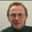
\includegraphics{fig/me.jpg}

\emph{Dyre Haugen} and \emph{Dyrehaugen} is Webian for \emph{Jon Martin} -
self-owned Globian, Webian, Norwegian and Canarian with
a background from industrial research policy, urban planning and
economic development consulting on global, regional and urban scales.
I am deeply concerned about the (insane) way
humanity (i.e.~capitalism) interfere with nature.
In an effort to gain insights in how and why this happens
stuff is collected from around the web and put together
in a linked set of web-sites.
The sites are operated as personal notebooks.
However, these days things can be easily published to the
benefit of others concerned with the same issues.
But be aware - this is not polished for presentation or
peer-reviewed for exactness.
I offer you just to have a look at my `work-desk' as it appears in the moment.
Any comment or suggestion can be mailed to \href{mailto:dyrehaugen@gmail.com}{\nolinkurl{dyrehaugen@gmail.com}}
You can follow me on twitter as @dyrehaugen.
Thanks for visiting!

\hypertarget{news}{%
\chapter{NEWS}\label{news}}

\hypertarget{climate-finance-shadow-report-2020}{%
\section{210102 Climate Finance Shadow Report 2020}\label{climate-finance-shadow-report-2020}}

Oxfam has released this report with subtitle \emph{Asessing progress towards the \$100 billion commitment}
Progress is NOT in line with need or pledges.

\begin{quote}
Climate change could undo decades of progress in development and dramatically increase global inequalities. There is an urgent need for climate finance to help countries cope and adapt.
Over a decade ago, developed countries committed to mobilize \$100bn per year by 2020 to support developing countries to adapt and reduce their emissions. The goal is a critical part of the Paris Agreement.
As 2020 draws to a close, Oxfam's Climate Finance Shadow Report 2020 offers an assessment of progress towards the \$100bn goal.
\end{quote}

\begin{quote}
Based on 2017--18 reported numbers, developed countries are likely to claim they are on track to meet
the \$100bn goal. And on their own terms, they may be. But how the goal is met is as important as whether
it is met. The dubious veracity of reported numbers, the extent to which climate finance is increasing
developing country indebtedness, and the enduring gap in support for adaptation, LDCs and SIDS, are grave
concerns. Meeting the \$100bn goal on these terms would be cause for concern, not celebration.
\end{quote}

\href{https://www.oxfam.org/en/research/climate-finance-shadow-report-2020}{Oxfam Report}
\href{/pdf/Oxfam_2020_Climate_Finance_Shadow_Report.pdf}{(pdf)}

  \bibliography{book.bib,packages.bib}

\end{document}
